\chapter{Conectividad fuerte}

\index{grafo fuertemente conexo}

En un grafo dirigido,
los bordes se pueden recorrer en una sola dirección,
por lo que incluso si el grafo está conectado,
esto no garantiza que haya
un camino de un nodo a otro nodo.
Por esta razón, es significativo definir un nuevo concepto
que requiere más que conectividad.

Un grafo es \key{fuertemente conexo}
si hay un camino desde cualquier nodo a todos
los demás nodos del grafo.
Por ejemplo, en la siguiente imagen,
el grafo izquierdo está fuertemente conectado
mientras que el grafo derecho no.

\begin{center}
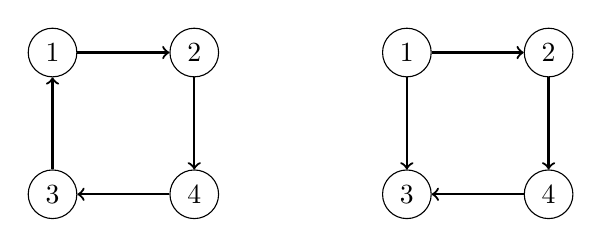
\begin{tikzpicture}[scale=0.9]
\node[draw, circle] (1) at (1,1) {$1$};
\node[draw, circle] (2) at (3,1) {$2$};
\node[draw, circle] (3) at (1,-1) {$3$};
\node[draw, circle] (4) at (3,-1) {$4$};

\path[draw,thick,->] (1) -- (2);
\path[draw,thick,->] (2) -- (4);
\path[draw,thick,->] (4) -- (3);
\path[draw,thick,->] (3) -- (1);

\node[draw, circle] (1b) at (6,1) {$1$};
\node[draw, circle] (2b) at (8,1) {$2$};
\node[draw, circle] (3b) at (6,-1) {$3$};
\node[draw, circle] (4b) at (8,-1) {$4$};

\path[draw,thick,->] (1b) -- (2b);
\path[draw,thick,->] (2b) -- (4b);
\path[draw,thick,->] (4b) -- (3b);
\path[draw,thick,->] (1b) -- (3b);
\end{tikzpicture}
\end{center}

El grafo derecho no está fuertemente conectado
porque, por ejemplo, no hay ningún camino
desde el nodo 2 al nodo 1.

\index{componente fuertemente conexo}
\index{grafo de componentes}

Los \key{componentes fuertemente conexos}
de un grafo dividen el grafo en partes fuertemente conectadas
que son lo más grandes posible.
Los componentes fuertemente conexos forman un
grafo \key{de componentes} acíclico que representa
la estructura profunda del grafo original.

Por ejemplo, para el grafo
\begin{center}
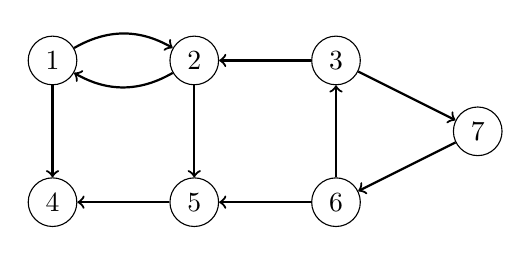
\begin{tikzpicture}[scale=0.9,label distance=-2mm]
\node[draw, circle] (1) at (-1,1) {$7$};
\node[draw, circle] (2) at (-3,2) {$3$};
\node[draw, circle] (4) at (-5,2) {$2$};
\node[draw, circle] (6) at (-7,2) {$1$};
\node[draw, circle] (3) at (-3,0) {$6$};
\node[draw, circle] (5) at (-5,0) {$5$};
\node[draw, circle] (7) at (-7,0) {$4$};

\path[draw,thick,->] (2) -- (1);
\path[draw,thick,->] (1) -- (3);
\path[draw,thick,->] (3) -- (2);
\path[draw,thick,->] (2) -- (4);
\path[draw,thick,->] (3) -- (5);
\path[draw,thick,->] (4) edge [bend left] (6);
\path[draw,thick,->] (6) edge [bend left] (4);
\path[draw,thick,->] (4) -- (5);
\path[draw,thick,->] (5) -- (7);
\path[draw,thick,->] (6) -- (7);
\end{tikzpicture}
\end{center}
los componentes fuertemente conexos son los siguientes:
\begin{center}
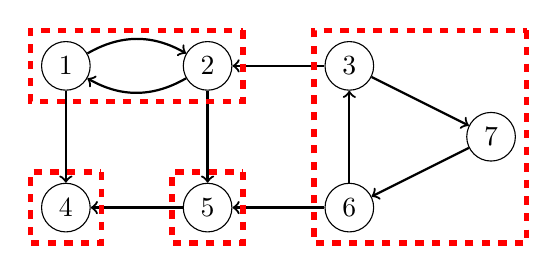
\begin{tikzpicture}[scale=0.9]
\node[draw, circle] (1) at (-1,1) {$7$};
\node[draw, circle] (2) at (-3,2) {$3$};
\node[draw, circle] (4) at (-5,2) {$2$};
\node[draw, circle] (6) at (-7,2) {$1$};
\node[draw, circle] (3) at (-3,0) {$6$};
\node[draw, circle] (5) at (-5,0) {$5$};
\node[draw, circle] (7) at (-7,0) {$4$};

\path[draw,thick,->] (2) -- (1);
\path[draw,thick,->] (1) -- (3);
\path[draw,thick,->] (3) -- (2);
\path[draw,thick,->] (2) -- (4);
\path[draw,thick,->] (3) -- (5);
\path[draw,thick,->] (4) edge [bend left] (6);
\path[draw,thick,->] (6) edge [bend left] (4);
\path[draw,thick,->] (4) -- (5);
\path[draw,thick,->] (5) -- (7);
\path[draw,thick,->] (6) -- (7);

\draw [red,thick,dashed,line width=2pt] (-0.5,2.5) rectangle (-3.5,-0.5);
\draw [red,thick,dashed,line width=2pt] (-4.5,2.5) rectangle (-7.5,1.5);
\draw [red,thick,dashed,line width=2pt] (-4.5,0.5) rectangle (-5.5,-0.5);
\draw [red,thick,dashed,line width=2pt] (-6.5,0.5) rectangle (-7.5,-0.5);
\end{tikzpicture}
\end{center}
El grafo de componentes correspondiente es el siguiente:
\begin{center}
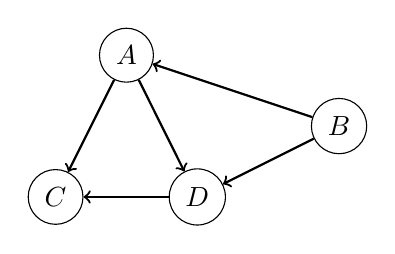
\begin{tikzpicture}[scale=0.9]
\node[draw, circle] (1) at (-3,1) {$B$};
\node[draw, circle] (2) at (-6,2) {$A$};
\node[draw, circle] (3) at (-5,0) {$D$};
\node[draw, circle] (4) at (-7,0) {$C$};

\path[draw,thick,->] (1) -- (2);
\path[draw,thick,->] (1) -- (3);
\path[draw,thick,->] (2) -- (3);
\path[draw,thick,->] (2) -- (4);
\path[draw,thick,->] (3) -- (4);
\end{tikzpicture}
\end{center}
Los componentes son $A=\{1,2\}$,
$B=\{3,6,7\}$, $C=\{4\}$ y $D=\{5\}$.

Un grafo de componentes es un grafo dirigido acíclico,
por lo que es más fácil de procesar que el grafo original.
Dado que el grafo no contiene ciclos,
siempre podemos construir una ordenación topológica y
utilizar técnicas de programación dinámica como las
que se presentan en el Capítulo 16.

\section{Algoritmo de Kosaraju}

\index{algoritmo de Kosaraju}

El \key{algoritmo de Kosaraju}\footnote{Según \cite{aho83},
S. R. Kosaraju inventó este algoritmo en 1978
pero no lo publicó. En 1981, el mismo algoritmo fue redescubierto
y publicado por M. Sharir \cite{sha81}.} es un método eficiente
para encontrar los componentes fuertemente conexos
de un grafo dirigido.
El algoritmo realiza dos búsquedas en profundidad:
la primera búsqueda construye una lista de nodos
de acuerdo con la estructura del grafo,
y la segunda búsqueda forma los componentes fuertemente conexos.

\subsubsection{Búsqueda 1}
La primera fase del algoritmo de Kosaraju construye
una lista de nodos en el orden en que una
búsqueda en profundidad los procesa.
El algoritmo recorre los nodos,
y comienza una búsqueda en profundidad en cada
nodo sin procesar.
Cada nodo se agregará a la lista
después de haber sido procesado.

En el gráfico de ejemplo, los nodos se procesan
en el siguiente orden:
\begin{center}
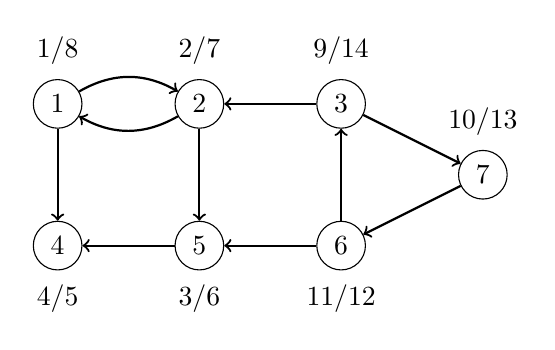
\begin{tikzpicture}[scale=0.9,label distance=-2mm]
\node[draw, circle] (1) at (-1,1) {$7$};
\node[draw, circle] (2) at (-3,2) {$3$};
\node[draw, circle] (4) at (-5,2) {$2$};
\node[draw, circle] (6) at (-7,2) {$1$};
\node[draw, circle] (3) at (-3,0) {$6$};
\node[draw, circle] (5) at (-5,0) {$5$};
\node[draw, circle] (7) at (-7,0) {$4$};

\node at (-7,2.75) {$1/8$};
\node at (-5,2.75) {$2/7$};
\node at (-3,2.75) {$9/14$};
\node at (-7,-0.75) {$4/5$};
\node at (-5,-0.75) {$3/6$};
\node at (-3,-0.75) {$11/12$};
\node at (-1,1.75) {$10/13$};

\path[draw,thick,->] (2) -- (1);
\path[draw,thick,->] (1) -- (3);
\path[draw,thick,->] (3) -- (2);
\path[draw,thick,->] (2) -- (4);
\path[draw,thick,->] (3) -- (5);
\path[draw,thick,->] (4) edge [bend left] (6);
\path[draw,thick,->] (6) edge [bend left] (4);
\path[draw,thick,->] (4) -- (5);
\path[draw,thick,->] (5) -- (7);
\path[draw,thick,->] (6) -- (7);
\end{tikzpicture}
\end{center}

La notación $x/y$ significa que
el procesamiento del nodo comenzó
en el tiempo $x$ y terminó en el tiempo $y$.
Por lo tanto, la lista correspondiente es la siguiente:

\begin{tabular}{ll}
\\
nodo & tiempo de procesamiento \\
\hline
4 & 5 \\
5 & 6 \\
2 & 7 \\
1 & 8 \\
6 & 12 \\
7 & 13 \\
3 & 14 \\
\\
\end{tabular}
% 
% En la segunda fase del algoritmo,
% los nodos se procesarán
% en orden inverso: $[3,7,6,1,2,5,4]$.

\subsubsection{Búsqueda 2}

La segunda fase del algoritmo
forma los componentes fuertemente conectados
del gráfico.
Primero, el algoritmo invierte cada
borde en el gráfico.
Esto garantiza que durante la segunda búsqueda,
siempre encontraremos componentes fuertemente conectados
que no tienen nodos adicionales.

Después de invertir los bordes,
el gráfico de ejemplo es el siguiente:
\begin{center}
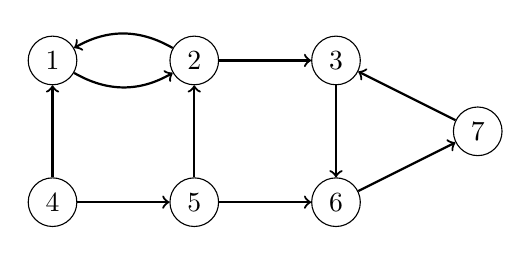
\begin{tikzpicture}[scale=0.9,label distance=-2mm]
\node[draw, circle] (1) at (-1,1) {$7$};
\node[draw, circle] (2) at (-3,2) {$3$};
\node[draw, circle] (4) at (-5,2) {$2$};
\node[draw, circle] (6) at (-7,2) {$1$};
\node[draw, circle] (3) at (-3,0) {$6$};
\node[draw, circle] (5) at (-5,0) {$5$};
\node[draw, circle] (7) at (-7,0) {$4$};

\path[draw,thick,<-] (2) -- (1);
\path[draw,thick,<-] (1) -- (3);
\path[draw,thick,<-] (3) -- (2);
\path[draw,thick,<-] (2) -- (4);
\path[draw,thick,<-] (3) -- (5);
\path[draw,thick,<-] (4) edge [bend left] (6);
\path[draw,thick,<-] (6) edge [bend left] (4);
\path[draw,thick,<-] (4) -- (5);
\path[draw,thick,<-] (5) -- (7);
\path[draw,thick,<-] (6) -- (7);
\end{tikzpicture}
\end{center}

Después de esto, el algoritmo recorre
la lista de nodos creada por la primera búsqueda,
en orden \emph{inverso}.
Si un nodo no pertenece a un componente,
el algoritmo crea un nuevo componente
y comienza una búsqueda en profundidad
que agrega todos los nodos nuevos encontrados durante la búsqueda
al nuevo componente.

En el gráfico de ejemplo, el primer componente
comienza en el nodo 3:

\begin{center}
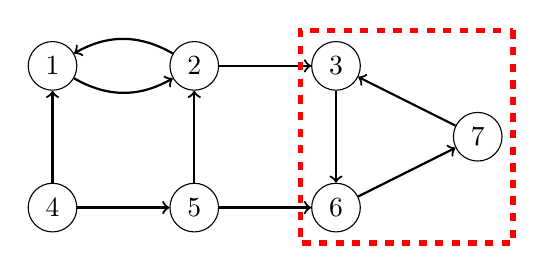
\begin{tikzpicture}[scale=0.9,label distance=-2mm]
\node[draw, circle] (1) at (-1,1) {$7$};
\node[draw, circle] (2) at (-3,2) {$3$};
\node[draw, circle] (4) at (-5,2) {$2$};
\node[draw, circle] (6) at (-7,2) {$1$};
\node[draw, circle] (3) at (-3,0) {$6$};
\node[draw, circle] (5) at (-5,0) {$5$};
\node[draw, circle] (7) at (-7,0) {$4$};

\path[draw,thick,<-] (2) -- (1);
\path[draw,thick,<-] (1) -- (3);
\path[draw,thick,<-] (3) -- (2);
\path[draw,thick,<-] (2) -- (4);
\path[draw,thick,<-] (3) -- (5);
\path[draw,thick,<-] (4) edge [bend left] (6);
\path[draw,thick,<-] (6) edge [bend left] (4);
\path[draw,thick,<-] (4) -- (5);
\path[draw,thick,<-] (5) -- (7);
\path[draw,thick,<-] (6) -- (7);

\draw [red,thick,dashed,line width=2pt] (-0.5,2.5) rectangle (-3.5,-0.5);
\end{tikzpicture}
\end{center}

Tenga en cuenta que dado que todos los bordes están invertidos,
el componente no ''se filtra'' a otras partes del gráfico.

\begin{samepage}
Los siguientes nodos en la lista son los nodos 7 y 6,
pero ya pertenecen a un componente,
por lo que el siguiente nuevo componente comienza en el nodo 1:

\begin{center}
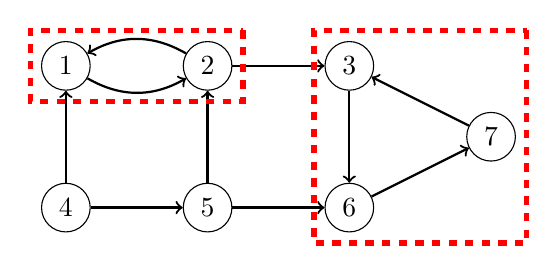
\begin{tikzpicture}[scale=0.9,label distance=-2mm]
\node[draw, circle] (1) at (-1,1) {$7$};
\node[draw, circle] (2) at (-3,2) {$3$};
\node[draw, circle] (4) at (-5,2) {$2$};
\node[draw, circle] (6) at (-7,2) {$1$};
\node[draw, circle] (3) at (-3,0) {$6$};
\node[draw, circle] (5) at (-5,0) {$5$};
\node[draw, circle] (7) at (-7,0) {$4$};

\path[draw,thick,<-] (2) -- (1);
\path[draw,thick,<-] (1) -- (3);
\path[draw,thick,<-] (3) -- (2);
\path[draw,thick,<-] (2) -- (4);
\path[draw,thick,<-] (3) -- (5);
\path[draw,thick,<-] (4) edge [bend left] (6);
\path[draw,thick,<-] (6) edge [bend left] (4);
\path[draw,thick,<-] (4) -- (5);
\path[draw,thick,<-] (5) -- (7);
\path[draw,thick,<-] (6) -- (7);



\draw [red,thick,dashed,line width=2pt] (-0.5,2.5) rectangle (-3.5,-0.5);
\draw [red,thick,dashed,line width=2pt] (-4.5,2.5) rectangle (-7.5,1.5);
%\draw [red,thick,dashed,line width=2pt] (-4.5,0.5) rectangle (-5.5,-0.5);
%\draw [red,thick,dashed,line width=2pt] (-6.5,0.5) rectangle (-7.5,-0.5);
\end{tikzpicture}
\end{center}
\end{samepage}

\begin{samepage}
Finalmente, el algoritmo procesa los nodos 5 y 4
que crean los componentes fuertemente conectados restantes:

\begin{center}
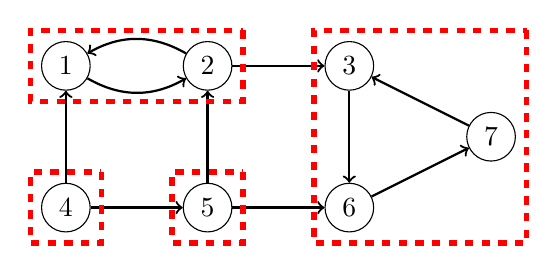
\begin{tikzpicture}[scale=0.9,label distance=-2mm]
\node[draw, circle] (1) at (-1,1) {$7$};
\node[draw, circle] (2) at (-3,2) {$3$};
\node[draw, circle] (4) at (-5,2) {$2$};
\node[draw, circle] (6) at (-7,2) {$1$};
\node[draw, circle] (3) at (-3,0) {$6$};
\node[draw, circle] (5) at (-5,0) {$5$};
\node[draw, circle] (7) at (-7,0) {$4$};

\path[draw,thick,<-] (2) -- (1);
\path[draw,thick,<-] (1) -- (3);
\path[draw,thick,<-] (3) -- (2);
\path[draw,thick,<-] (2) -- (4);
\path[draw,thick,<-] (3) -- (5);
\path[draw,thick,<-] (4) edge [bend left] (6);
\path[draw,thick,<-] (6) edge [bend left] (4);
\path[draw,thick,<-] (4) -- (5);
\path[draw,thick,<-] (5) -- (7);
\path[draw,thick,<-] (6) -- (7);

\draw [red,thick,dashed,line width=2pt] (-0.5,2.5) rectangle (-3.5,-0.5);
\draw [red,thick,dashed,line width=2pt] (-4.5,2.5) rectangle (-7.5,1.5);
\draw [red,thick,dashed,line width=2pt] (-4.5,0.5) rectangle (-5.5,-0.5);
\draw [red,thick,dashed,line width=2pt] (-6.5,0.5) rectangle (-7.5,-0.5);
\end{tikzpicture}
\end{center}
\end{samepage}

La complejidad temporal del algoritmo es $O(n+m)$,
porque el algoritmo
realiza dos búsquedas en profundidad.

\section{Problema 2SAT}

\index{Problema 2SAT}

La conectividad fuerte también está relacionada con el
\key{problema 2SAT}\footnote{El algoritmo presentado aquí fue
introducido en \cite{asp79}.
También existe otro algoritmo conocido de tiempo lineal \cite{eve75}
que se basa en el retroceso.}.
En este problema, se nos da una fórmula lógica
\[
(a_1 \lor b_1) \land (a_2 \lor b_2) \land \cdots \land (a_m \lor b_m),
\]
donde cada $a_i$ y $b_i$ es una variable lógica
($x_1,x_2,\ldots,x_n$)
o una negación de una variable lógica
($\lnot x_1, \lnot x_2, \ldots, \lnot x_n$).
Los símbolos ''$\land$'' y ''$\lor$'' denotan
operadores lógicos ''y'' y ''o''.
Nuestra tarea es asignar a cada variable un valor
para que la fórmula sea verdadera, o indicar
que esto no es posible.

Por ejemplo, la fórmula
\[
L_1 = (x_2 \lor \lnot x_1) \land
      (\lnot x_1 \lor \lnot x_2) \land
      (x_1 \lor x_3) \land
      (\lnot x_2 \lor \lnot x_3) \land
      (x_1 \lor x_4)
\]
es verdadera cuando las variables se asignan de la siguiente manera:

\[
\begin{cases}
x_1 = \textrm{falso} \\
x_2 = \textrm{falso} \\
x_3 = \textrm{verdadero} \\
x_4 = \textrm{verdadero} \\
\end{cases}
\]

Sin embargo, la fórmula
\[
L_2 = (x_1 \lor x_2) \land
      (x_1 \lor \lnot x_2) \land
      (\lnot x_1 \lor x_3) \land
      (\lnot x_1 \lor \lnot x_3)
\]
siempre es falsa, independientemente de cómo
asignemos los valores.
La razón de esto es que no podemos
elegir un valor para $x_1$
sin crear una contradicción.
Si $x_1$ es falso, tanto $x_2$ como $\lnot x_2$
deberían ser verdaderos, lo cual es imposible,
y si $x_1$ es verdadero, tanto $x_3$ como $\lnot x_3$
deberían ser verdaderos, lo cual también es imposible.

El problema 2SAT se puede representar como un gráfico
cuyos nodos corresponden a
variables $x_i$ y negaciones $\lnot x_i$,
y los bordes determinan las conexiones
entre las variables.
Cada par $(a_i \lor b_i)$ genera dos bordes:
$\lnot a_i \to b_i$ y $\lnot b_i \to a_i$.
Esto significa que si $a_i$ no se cumple,
$b_i$ debe cumplirse, y viceversa.

El gráfico para la fórmula $L_1$ es:
\\
\begin{center}
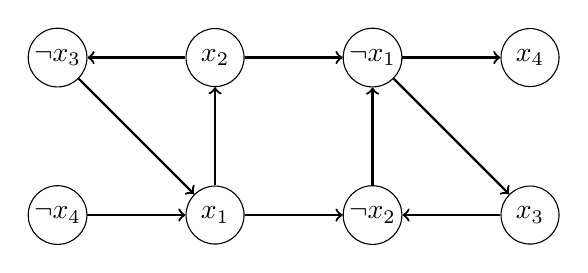
\begin{tikzpicture}[scale=1.0,minimum size=2pt]
\node[draw, circle, inner sep=1.3pt] (1) at (1,2) {$\lnot x_3$};
\node[draw, circle] (2) at (3,2) {$x_2$};
\node[draw, circle, inner sep=1.3pt] (3) at (1,0) {$\lnot x_4$};
\node[draw, circle] (4) at (3,0) {$x_1$};
\node[draw, circle, inner sep=1.3pt] (5) at (5,2) {$\lnot x_1$};
\node[draw, circle] (6) at (7,2) {$x_4$};
\node[draw, circle, inner sep=1.3pt] (7) at (5,0) {$\lnot x_2$};
\node[draw, circle] (8) at (7,0) {$x_3$};
 
\path[draw,thick,->] (1) -- (4);
\path[draw,thick,->] (4) -- (2);
\path[draw,thick,->] (2) -- (1);
\path[draw,thick,->] (3) -- (4);
\path[draw,thick,->] (2) -- (5);
\path[draw,thick,->] (4) -- (7);
\path[draw,thick,->] (5) -- (6);
\path[draw,thick,->] (5) -- (8);
\path[draw,thick,->] (8) -- (7);
\path[draw,thick,->] (7) -- (5);
\end{tikzpicture}
\end{center}
Y el gráfico para la fórmula $L_2$ es:
\\
\begin{center}
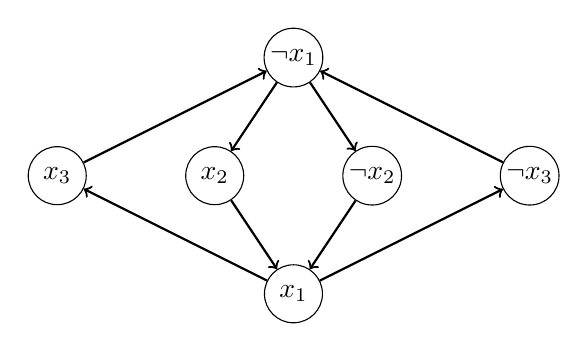
\begin{tikzpicture}[scale=1.0,minimum size=2pt]
\node[draw, circle] (1) at (1,2) {$x_3$};
\node[draw, circle] (2) at (3,2) {$x_2$};
\node[draw, circle, inner sep=1.3pt] (3) at (5,2) {$\lnot x_2$};
\node[draw, circle, inner sep=1.3pt] (4) at (7,2) {$\lnot x_3$};
\node[draw, circle, inner sep=1.3pt] (5) at (4,3.5) {$\lnot x_1$};
\node[draw, circle] (6) at (4,0.5) {$x_1$};
\path[draw,thick,->] (1) -- (5);
\path[draw,thick,->] (4) -- (5);
\path[draw,thick,->] (6) -- (1);
\path[draw,thick,->] (6) -- (4);
\path[draw,thick,->] (5) -- (2);
\path[draw,thick,->] (5) -- (3);
\path[draw,thick,->] (2) -- (6);
\path[draw,thick,->] (3) -- (6);
\end{tikzpicture}
\end{center}

La estructura del grafo nos dice si
es posible asignar los valores
de las variables para que
la fórmula sea verdadera.
Resulta que esto se puede hacer
exactamente cuando no hay nodos
$x_i$ y $\lnot x_i$ tales que
ambos nodos pertenezcan al
mismo componente fuertemente conectado.
Si hay tales nodos,
el grafo contiene
un camino desde $x_i$ a $\lnot x_i$
y también un camino desde $\lnot x_i$ a $x_i$,
por lo que tanto $x_i$ como $\lnot x_i$ deben ser verdaderos
lo cual no es posible.

En el grafo de la fórmula $L_1$
no hay nodos $x_i$ y $\lnot x_i$
tales que ambos nodos
pertenezcan al mismo componente fuertemente conectado,
por lo que existe una solución.
En el grafo de la fórmula $L_2$
todos los nodos pertenecen al mismo componente fuertemente conectado,
por lo que no existe una solución.

Si existe una solución, los valores para las variables
se pueden encontrar recorriendo los nodos del
grafo de componentes en un orden de clasificación topológica inverso.
En cada paso, procesamos un componente 
que no contiene aristas que conduzcan a un
componente no procesado.
Si las variables en el componente
no han sido asignadas valores,
sus valores serán determinados
de acuerdo con los valores en el componente,
y si ya tienen valores,
permanecen sin cambios.
El proceso continúa hasta que cada variable
ha sido asignado un valor.

El grafo de componentes para la fórmula $L_1$ es el siguiente:
\begin{center}
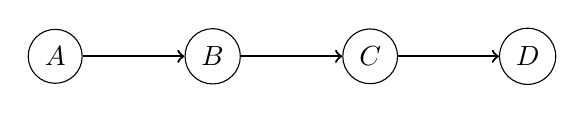
\begin{tikzpicture}[scale=1.0]
\node[draw, circle] (1) at (0,0) {$A$};
\node[draw, circle] (2) at (2,0) {$B$};
\node[draw, circle] (3) at (4,0) {$C$};
\node[draw, circle] (4) at (6,0) {$D$};

\path[draw,thick,->] (1) -- (2);
\path[draw,thick,->] (2) -- (3);
\path[draw,thick,->] (3) -- (4);
\end{tikzpicture}
\end{center}

Los componentes son
$A = \{\lnot x_4\}$,
$B = \{x_1, x_2, \lnot x_3\}$,
$C = \{\lnot x_1, \lnot x_2, x_3\}$ y
$D = \{x_4\}$.
Al construir la solución,
primero procesamos el componente $D$
donde $x_4$ se vuelve verdadero.
Después de esto, procesamos el componente $C$
donde $x_1$ y $x_2$ se vuelven falsos
y $x_3$ se vuelve verdadero.
Todas las variables han sido asignadas valores,
por lo que los componentes restantes $A$ y $B$
no cambian las variables.

Tenga en cuenta que este método funciona, porque el
grafo tiene una estructura especial:
si hay caminos desde el nodo $x_i$ al nodo $x_j$
y desde el nodo $x_j$ al nodo $\lnot x_j$,
entonces el nodo $x_i$ nunca se vuelve verdadero.
La razón de esto es que también hay
un camino desde el nodo $\lnot x_j$ al nodo $\lnot x_i$,
y tanto $x_i$ como $x_j$ se vuelven falsos.

\index{3SAT problem}

Un problema más difícil es el \key{3SAT problem},
donde cada parte de la fórmula es de la forma
$(a_i \lor b_i \lor c_i)$.
Este problema es NP-difícil, por lo que no se conoce ningún algoritmo eficiente
para resolver el problema.
